\documentclass[a4paper,11pt,oneside]{article}
\usepackage[utf8]{inputenc}
\usepackage{setspace}
\usepackage{hyperref}
\usepackage{graphicx}
\graphicspath{ {images/}}
\usepackage[left=0.5in, right=2in, bottom=1in, top=0.5in]{geometry}
\pagenumbering{arabic}
\renewcommand{\familydefault}{\sfdefault}
\begin{document}

\noindent\LARGE{\textbf{ Hrushikesh Budhale}}  \\
\vspace{0ex}
\noindent\hrulefill
\normalsize


\begin{center}
\vspace{-3ex}
\begin{tabular}{l r}
 Walchand College of Engineering,    & \hspace{2.5in} Contact: +91 9623928230\\
 Sangli-416415,                      & \hspace{2.5in} e-mail id: \href{mailto:hruhnb@email.com}{hruhnb@email.com} \\
 Maharashtra                         & \\
                                     & \hspace{2.5in} 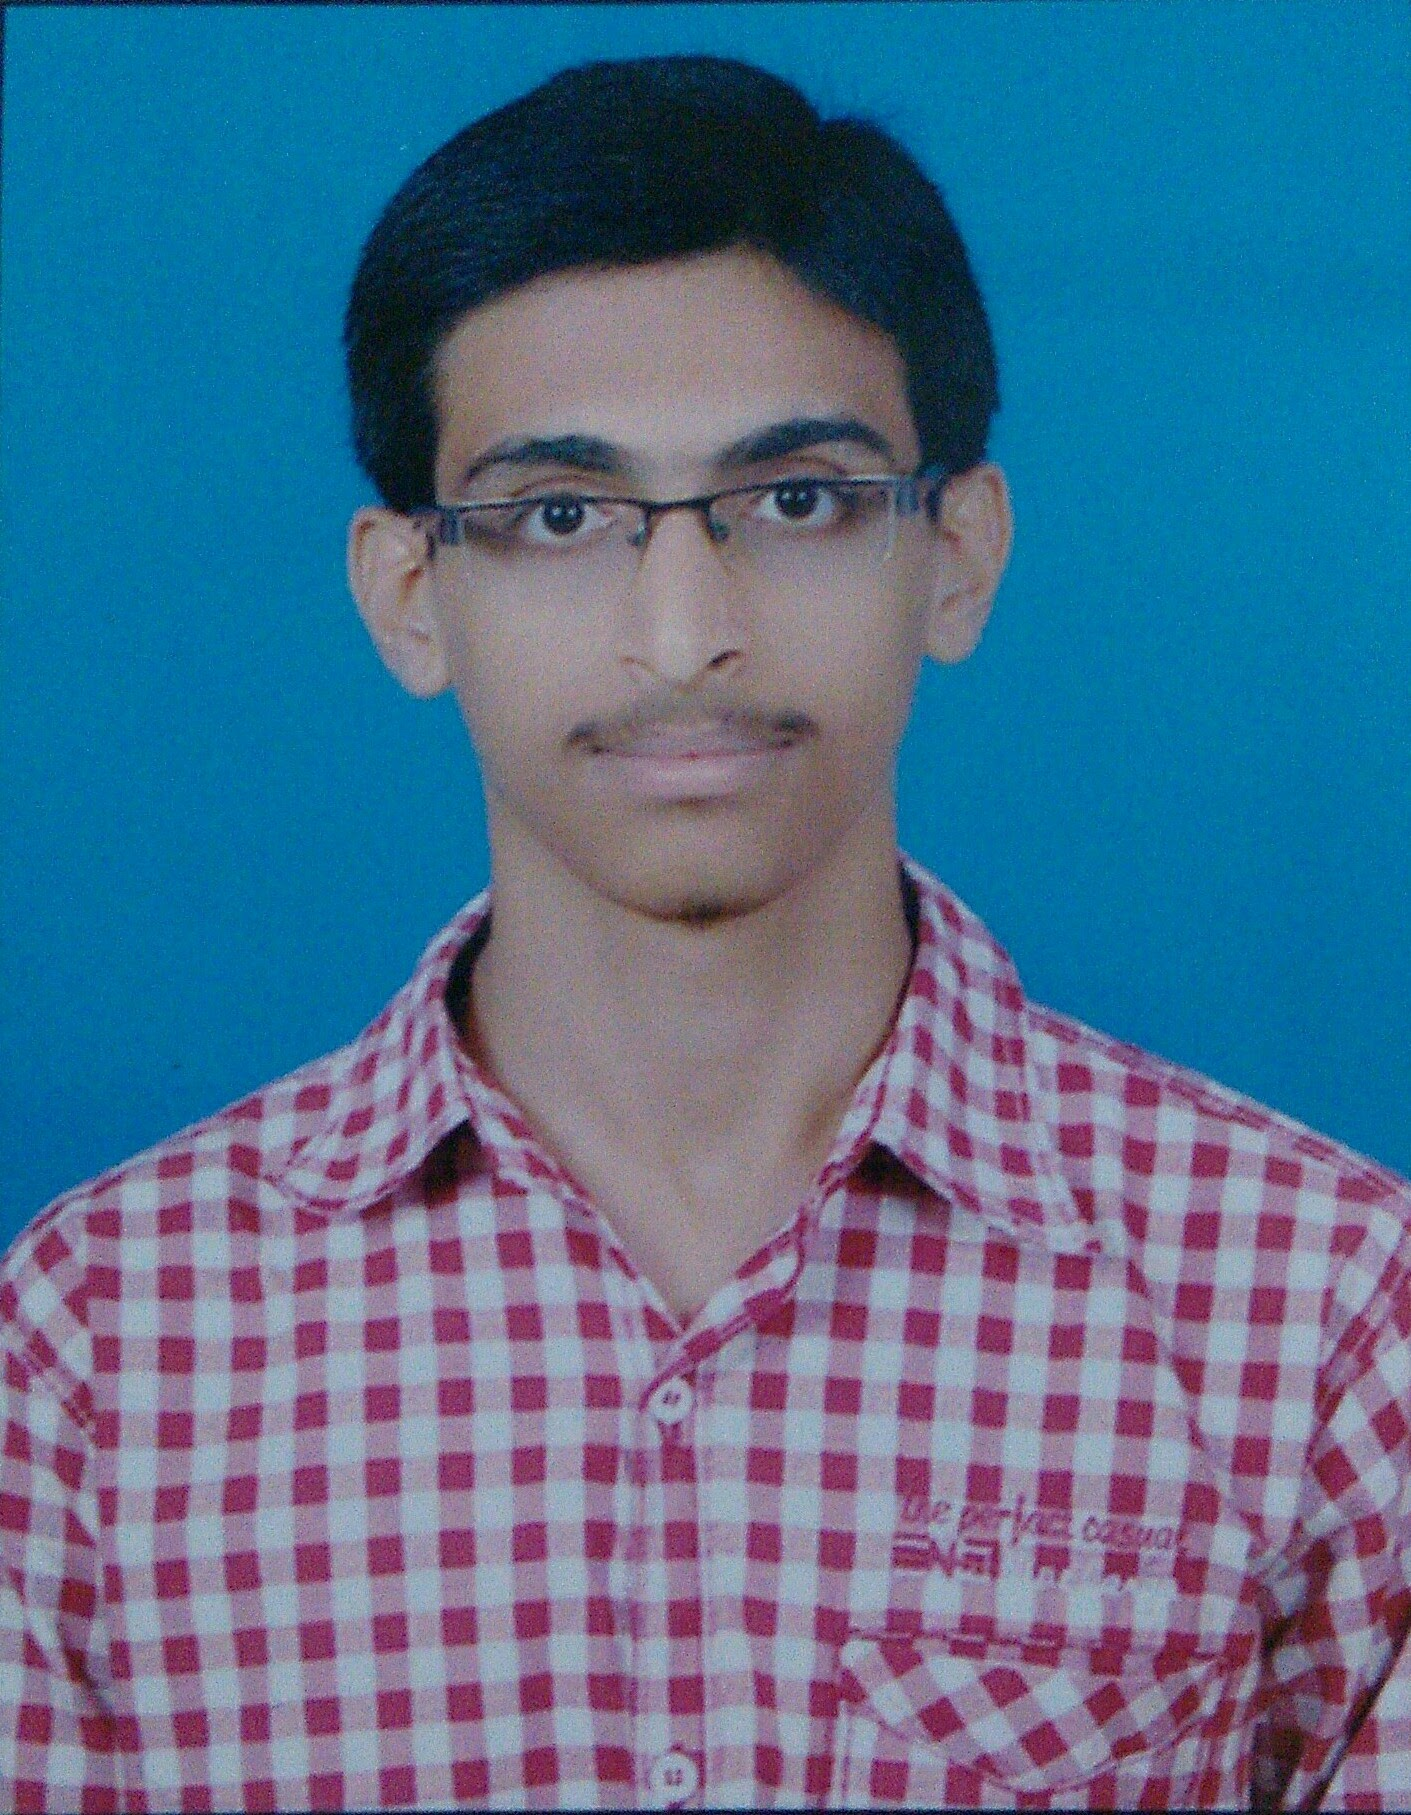
\includegraphics[scale=0.04]{id.jpg} \\
\end{tabular}
\end{center}

% \begin{flushright}
%     \includegraphics[scale=0.6]{Phillips} \\
% \end{flushright}

\noindent \begin{tabular}{@{} p{0.2\textwidth} p{\textwidth}}
     \textbf{\large{Objective}}
         & \large{Obtain an internship in  that will benefit from an advanced knowledge of} \\
         & \large{robotics and algorithmic programming skills.} \\ \\
         
     \textbf{\large{Education}}
         & \begin{tabular}[t]{ |l|c|l|l|l| }
                \hline
                \textbf{Degree} & \textbf{College/School} & \textbf{University} & \textbf{Passing} & \textbf{Pass} \\
                &  &  & \textbf{year} & \textbf{Percentage} \\
                \hline
                BTech & Walchand College of Engg., & Autonomous & 2018-19 & 8.01 \scriptsize{CGPA} \\ 
                & Sangli & & & \\ 
                \hline
                HSC & Shri Mhalsakant Vidyalaya,& Pune & 2014-15 & 82.86\%   \\ 
                & Chinchwad & & & \\ 
                \hline
                SSC & New English School, & Kolhapur & 2012-13 & 85.6\% \\ 
                & Satara & & & \\ 
                \hline
            
            \end{tabular}
            \vspace{2em} \\
            
 
 
\clearpage

\end{document}